\documentclass[12pt]{article}

\usepackage{setspace}
\usepackage{amsmath}
\usepackage{amsfonts}
\usepackage{graphicx}
\usepackage{float}
\addtolength{\oddsidemargin}{-.7in}
\addtolength{\evensidemargin}{-.7in}
\addtolength{\textwidth}{1.4in}
\usepackage{enumerate}
\onehalfspacing
\usepackage{geometry} % Required for customizing page layout

\usepackage{caption}
\usepackage{booktabs}

\usepackage{hyperref}
\hypersetup{
	pdfstartview = FitH,
	pdfauthor = {...},
	pdftitle = {...},
	pdfkeywords = {...; ...; ...; ...},
	colorlinks = true,
	linkcolor = blue,
	urlcolor = blue,
	citecolor = blue,
	linktocpage=true
}


\begin{document}

\section*{Appendix}
\subsection*{A1 - Bankruptcy frameworks in the US and EU}

The US Bankruptcy Code is structured into chapters, each corresponding to a different type of relief for debtors in financial distress. In particular, chapter 7 deals with liquidations and chapter 11 regulates the reorganization process. The European Union does not have a single bankruptcy code, but it has been working towards harmonizing insolvency proceedings across member states, based on the understanding that divergent insolvency laws create barriers across member states. As a result, the Harmonisation Directive\footnote{Directive (EU) 2019/1023 of the European Parliament and of the Council of 20 June 2019 on preventive restructuring frameworks, on discharge of debt and disqualifications, and on measures to increase the efficiency of procedures concerning restructuring, insolvency and discharge of debt.}  was published in June 2019, and member states are required to adopt the necessary legislative changes by July 2021 to comply with it. Although it does not completely standardize bankruptcy procedures, the directive outlines several principles that mirror the main features of chapter 7 and 11 of the US bankruptcy code. For the purpose of this discussion, it represents a valuable piece of information as it collects the set of principles that legislators aim to  institute in bankruptcy proceedings. \vspace{3mm} \\
Under both frameworks, the debtor is expected to file for insolvency – although creditors may petition the court to initiate bankruptcy proceedings against the debtor, this is not the norm. Hence, the decision to pursue reorganization or liquidation initially lies with the debtor. If the debtor decides to draft a reorganization plan, creditors may form committees and have their claims heard by courts. The European Union has a more debtor-friendly approach, meaning that creditors have less influence over the outcome of the proceedings, whereas the US system places more weight on the best interest of the creditors. However, it is often the case that a debtor has numerous creditors, which limits the influence of any individual creditor over the specifics of the bankruptcy proceedings. \vspace{3mm} \\
One exception to this rule, is that no dissenting creditor should be worse off under the proposed reorganization plan than it would be in case of liquidation. The EU Directive refers this as ‘best-interest-of-creditors’ test in OJ L 172/27, art. 49; whereas the US bankruptcy code establishes this principle in 11 U.S. Code § 1129.  If the reorganization plan fails this test, it may not receive the necessary court approval (the dissenting creditor is entitled to vote against it). In the context of the model, this becomes relevant when an asset-based borrower decides to file for reorganization. The lender cannot receive a lower payoff than it expects to see from the liquidation of collateral (although it might have to pay some legal fees). Thus, from the point of view of the asset-based lender it does not matter if the borrower wishes to continue operating after the bankruptcy have been resolved. As discussed in section ... I abstract from these cases altogether.  \vspace{3mm} \\
Creditors have even less influence when a borrower seeks to resolve financial distress through liquidation of its assets as it would be unrealistic to expect the firm to continue operating against the best judgement of its management. An important exception from this rule is when the debt is secured against the entire corporate entity. In this case, the creditor can take over the firm in case of default and may decide freely between reorganization and liquidation. Yet, cash-flow based lenders must take into account that in case of a default, they may only retrieve the liquidation value of the collateral.  This outcome could arise from mutual creditor-debtor agreement. Alternatively, it may reflect debtors' choice, possibly conflicting with the creditor's best interests. Hence, the risk premium on these loans will reflect the `Chapter 7 outcome’ too unless the lender deems that the probability of reorganization is negligible. 

\subsection*{A2 - Earnings based constraints and cash flow based lending}

\subsection*{A3 - Data appendix}
\subsubsection*{A3.1 - Compustat and Capital IQ}
Compustat is a comprehensive, financial database maintained by S\&P Global. It offers standardized firm-level information on publicly traded companies compiled from  financial statements, regulatory filings and other financial reports. I use the quarterly tables in Compustat North America which chiefly contains US and Canadian corporations. Moreover, I exclude financial corporations (SIC code 6000 to 6799) and utility providers (SIC code 4900-4999) from the sample. S\&P Capital IQ offers an extensive array of debt-level statistics. The two datasets can be conveniently connected via the unique firm a identifier (GVKEY), moreover Capital IQ covers most of the Compustat firms and yields consistent firm-level debt data after the aggregation of debt contracts. Although Capital IQ covers most major economies, I only focus on North American corporations, due to limitations introduced by Compustat.  \vspace{3mm} \\
Although both datasets provide high quality data, reporting differences necessitate some manipulation of the data. Since monetary variables are often reported in the native currency, I bring all observations to USD. Moreover, Capital IQ reports data points in different units (units, thousands or millions). To be consistent to Compustat, I bring all observations to millions of units. It must also be ensured that each observation is uniquely identified by the combination of year, quarter, and debt ID. This may be violated for various reasons, for instance, debt facilities are often reported twice (once with the total accessible debt and once with the currently outstanding amount). Moreover, subsidiaries are also often included in the data. I exclude these to maintain observations at the highest consolidation level. \vspace{3mm} \\
In some instances, debt contracts go missing only to reappear a few quarter later. If this gap between observations is no more the 4 quarter, I use linear interpolation to fill up the data. However, these cases are relatively rare, they only amount to approximately 7\% of the total sample. To ensure the alignment of consistent observations, I aggregate debt-level data from CapitalIQ to the firm level and cross-reference it with the debt information reported by Compustat. I drop any observations where there is a disparity of more than 20\% between the two datasets. This amounts to around 8\% of the sample. The following tables summarize Compustat and Capital IQ variables, including their original names and definitions in these datasets.

\begin{table}[htbp]
\centering
\caption{Compustat variable definitions}
\label{tab:Compustat variable definitions}
\renewcommand{\arraystretch}{1.5} % Increase the vertical spacing of rows
\resizebox{\textwidth}{!}{%
\begin{tabular}{lp{5cm}p{7cm}} 
\toprule
Variable & Compustat Definition & Description \\
\midrule
Total debt & dlcq+dlttq & Long-Term Debt + Debt in Current Liabilities \\
Leverage & (dlcq+dlttq)/atq & Total debt / Total Assets \\
Collateral & ppentq+invtq+rectq & Total Property, Plant and Equipment (net) + Receivables + Inventory \\
Pledgeability & (ppentq+invtq+rectq)/atq & Collateral / Total Assets \\
Interest coverage & oibdpq / xintq & Operating income before depreciation / Interest related expenses \\
Investment & capxq-sppeq & Capital expenditures - Sale of Property \\
Investment rate & (capxy - sppey) / l.ppegtq & Investment / Lag of Total Property, Plant and Equipment (gross) \\
Equity & atq-ltq & Total assets / Total liabilities \\
Net debt & dlcq+dltq-chq & Total debt - Cash Holdings \\
Liquidity & chq/atq & Cash Holdings / Total Assets \\
Assets & atq & Total Assets (book value) \\
Liabilities & ltq & Liabilities (book value) \\
Revenue & revtq & Total quarter revenue \\
Employees & emp & Total number of employees (thousands) \\
Industry spec. & sic & SIC code \\
Credit rating & spcsrc & S\&P credit rating \\
Added value & revtq - cogsq & Total revenue - Input costs \\
Productivity & $\frac{revtq - cogsq}{ppegtq^{1/3} + emp^{2/3}}$ & Added value / Assets and Employees \\
Age & defined from Capital IQ & Current year - Year founded + 1 \\
\bottomrule
\end{tabular}
}
\end{table}

\newpage

\begin{table}[htbp]
\centering
\caption{Capital IQ Variables}
\label{tab:capital_iq_variables}
\begin{tabular}{ll}
\toprule
Variable & Capital IQ \\
\midrule
Loan value & dataitemvalue \\
Decimal of the value & unittypeId \\
Currency of issuance & issuedCurrencyId \vspace{3mm} \\
\multicolumn{2}{l}{\textbf{Used for classification}} \\
Description of the contract & capitalstructuredescription \\
Type of the debt contract & capitalstructuresubtypeid \\
Debt description in text & descriptiontext \\
Secured dummy & securedtypeid \\
Seniority & leveltypeid \vspace{3mm} \\
\multicolumn{2}{l}{\textbf{Firm-level aggregated variables}} \\
Total debt value & Sum of all contracts value \\
AB value & Sum of all AB debt \\
CF value & Sum of all CF debt \\
CF share & CF value / Total debt \\
\bottomrule
\end{tabular}
\end{table}

\subsubsection*{A3.2 - Matching capitalIQ and ORBIS}
There is no common firm-identifier that could be used to directly match observations in ORBIS and CapitalIQ. Therefore, I resort to finding matches based on company-names and other observable characteristics, such as the location of headquarters (i.e. country, zip code and street name) company fax and website. This exercise is complicated by the occasional reporting differences adapted by these data providers. In the following, I detail the matching strategy that is used to connect CapitalIQ and ORBIS. \vspace{3mm} \\
First, I identify exact matches of company-names (disregarding capitalization). This pairs up 43\% of the observations. Second, I identify the most often recurring expressions in company names - these are typically descriptions of the organizational form, such as "limited", "ltd.", "corporation", "corp.". Removing these matches 54\% percent of observations. Third, I identify potential matches via website, zipcode, address and fax information - these yield additional matches of approximately 9\% of the dataset. Fourth, I find the closest match to each company name based on the Jaro-Winkler distance. If this metric is under under 0.15, I identify the pairing as a genuine match.\footnote{This cutoff is based on the frequency the string distance matching choosing different matches than identified by previous steps.} \vspace{3mm} \\
Finally, I consider the information on the main country of residence for the company. A company under the same name may be reported to reside in a different country for the following reasons: \textit{a)} foreign subsidiaries of multinational companies reported under the same name \textit{b)} the same multinationals reported to different countries and \textit{c)} different companies that coincidentally have the same name. Only in case \textit{b)} would it be desirable to identify a pairing as a genuine match. Since there is no straightforward way to differentiate between these cases, I only accept matches that report the same country as the location of their headquarters. This provides a sanity-check for the matching strategy, albeit at the expense of possibly discarding some genuine matches. Overall, I manage to match 77\% of firms present in capitalIQ to ORBIS.

\newpage
\subsection*{A4 - Further statistics}
\subsubsection*{A4.1 - Compustat and Capital IQ evidence}
Table 3. details measures the difference between AB-reliant and CF-reliant firms. The t-statistics show that firm that hols a positive share of CF-based debt on their portfolio are significantly bigger than firms that do not. 

\begin{table}[H]
\centering
\resizebox{\textwidth}{!}{%
\begin{tabular}{l|rrrr}
\multicolumn{5}{l}{\textbf{Firm-Level - ABL vs CFL borrowers}} \\
\hline
&  \textbf{Mean-CFL} & \textbf{ Mean-ABL} &\textbf{ t-stat} & \textbf{p-value} \\ 
Total Assets (millions USD) & 7462.63 & 603.24 & 86.84 & 0.00 \\ 
Qtr. Revenue (millions USD) & 1506.07 & 132.81 & 76.14 & 0.00 \\ 
Employment (thousands) & 16.92 & 2.61 & 55.62 & 0.00 \\ 
Age (years) & 49.36 & 32.93 & 88.68 & 0.00 \\ 
Total debt (millions USD) & 2720.27 & 147.89 & 86.92 & 0.00 \\ 
Leverage & 0.43 & 0.21 & 144.01 & 0.00 \\ 
Productivity & 0.04 & 0.02 & 95.51 & 0.00 \\ 
\hline
\end{tabular}
}
\caption{\small Summary Statistics: a comparison of average values of ABL firms and CFL firms, the P-value reports the probability of the two sample averages being same.} 
\end{table}

\noindent In line with previous findings of Lian and Ma (2021) and Öztürk (2022), the total outstanding debt volume that can be classified as CF-based is relatively stable around 75\%. However, starting from 2019, this share drops significantly - from 79\% in 2018Q4 to 71\% 2019Q4 - and it does not fully recover until the end of the sample. I cannot compare this result to previous studies, since their results do not extend to this period. It is not clear what causes this abrupt shift in aggregate CFL reliance. One explanation could be the Covid-induced economic crisis. However, this leaves the initial drop. which happen before the pandemic had a substantial impact on North American economies unexplained. 

\begin{figure}[H]  % [h] indicates placing the image here
    \centering
    \caption{The share of cash flow based debt to total debt}
    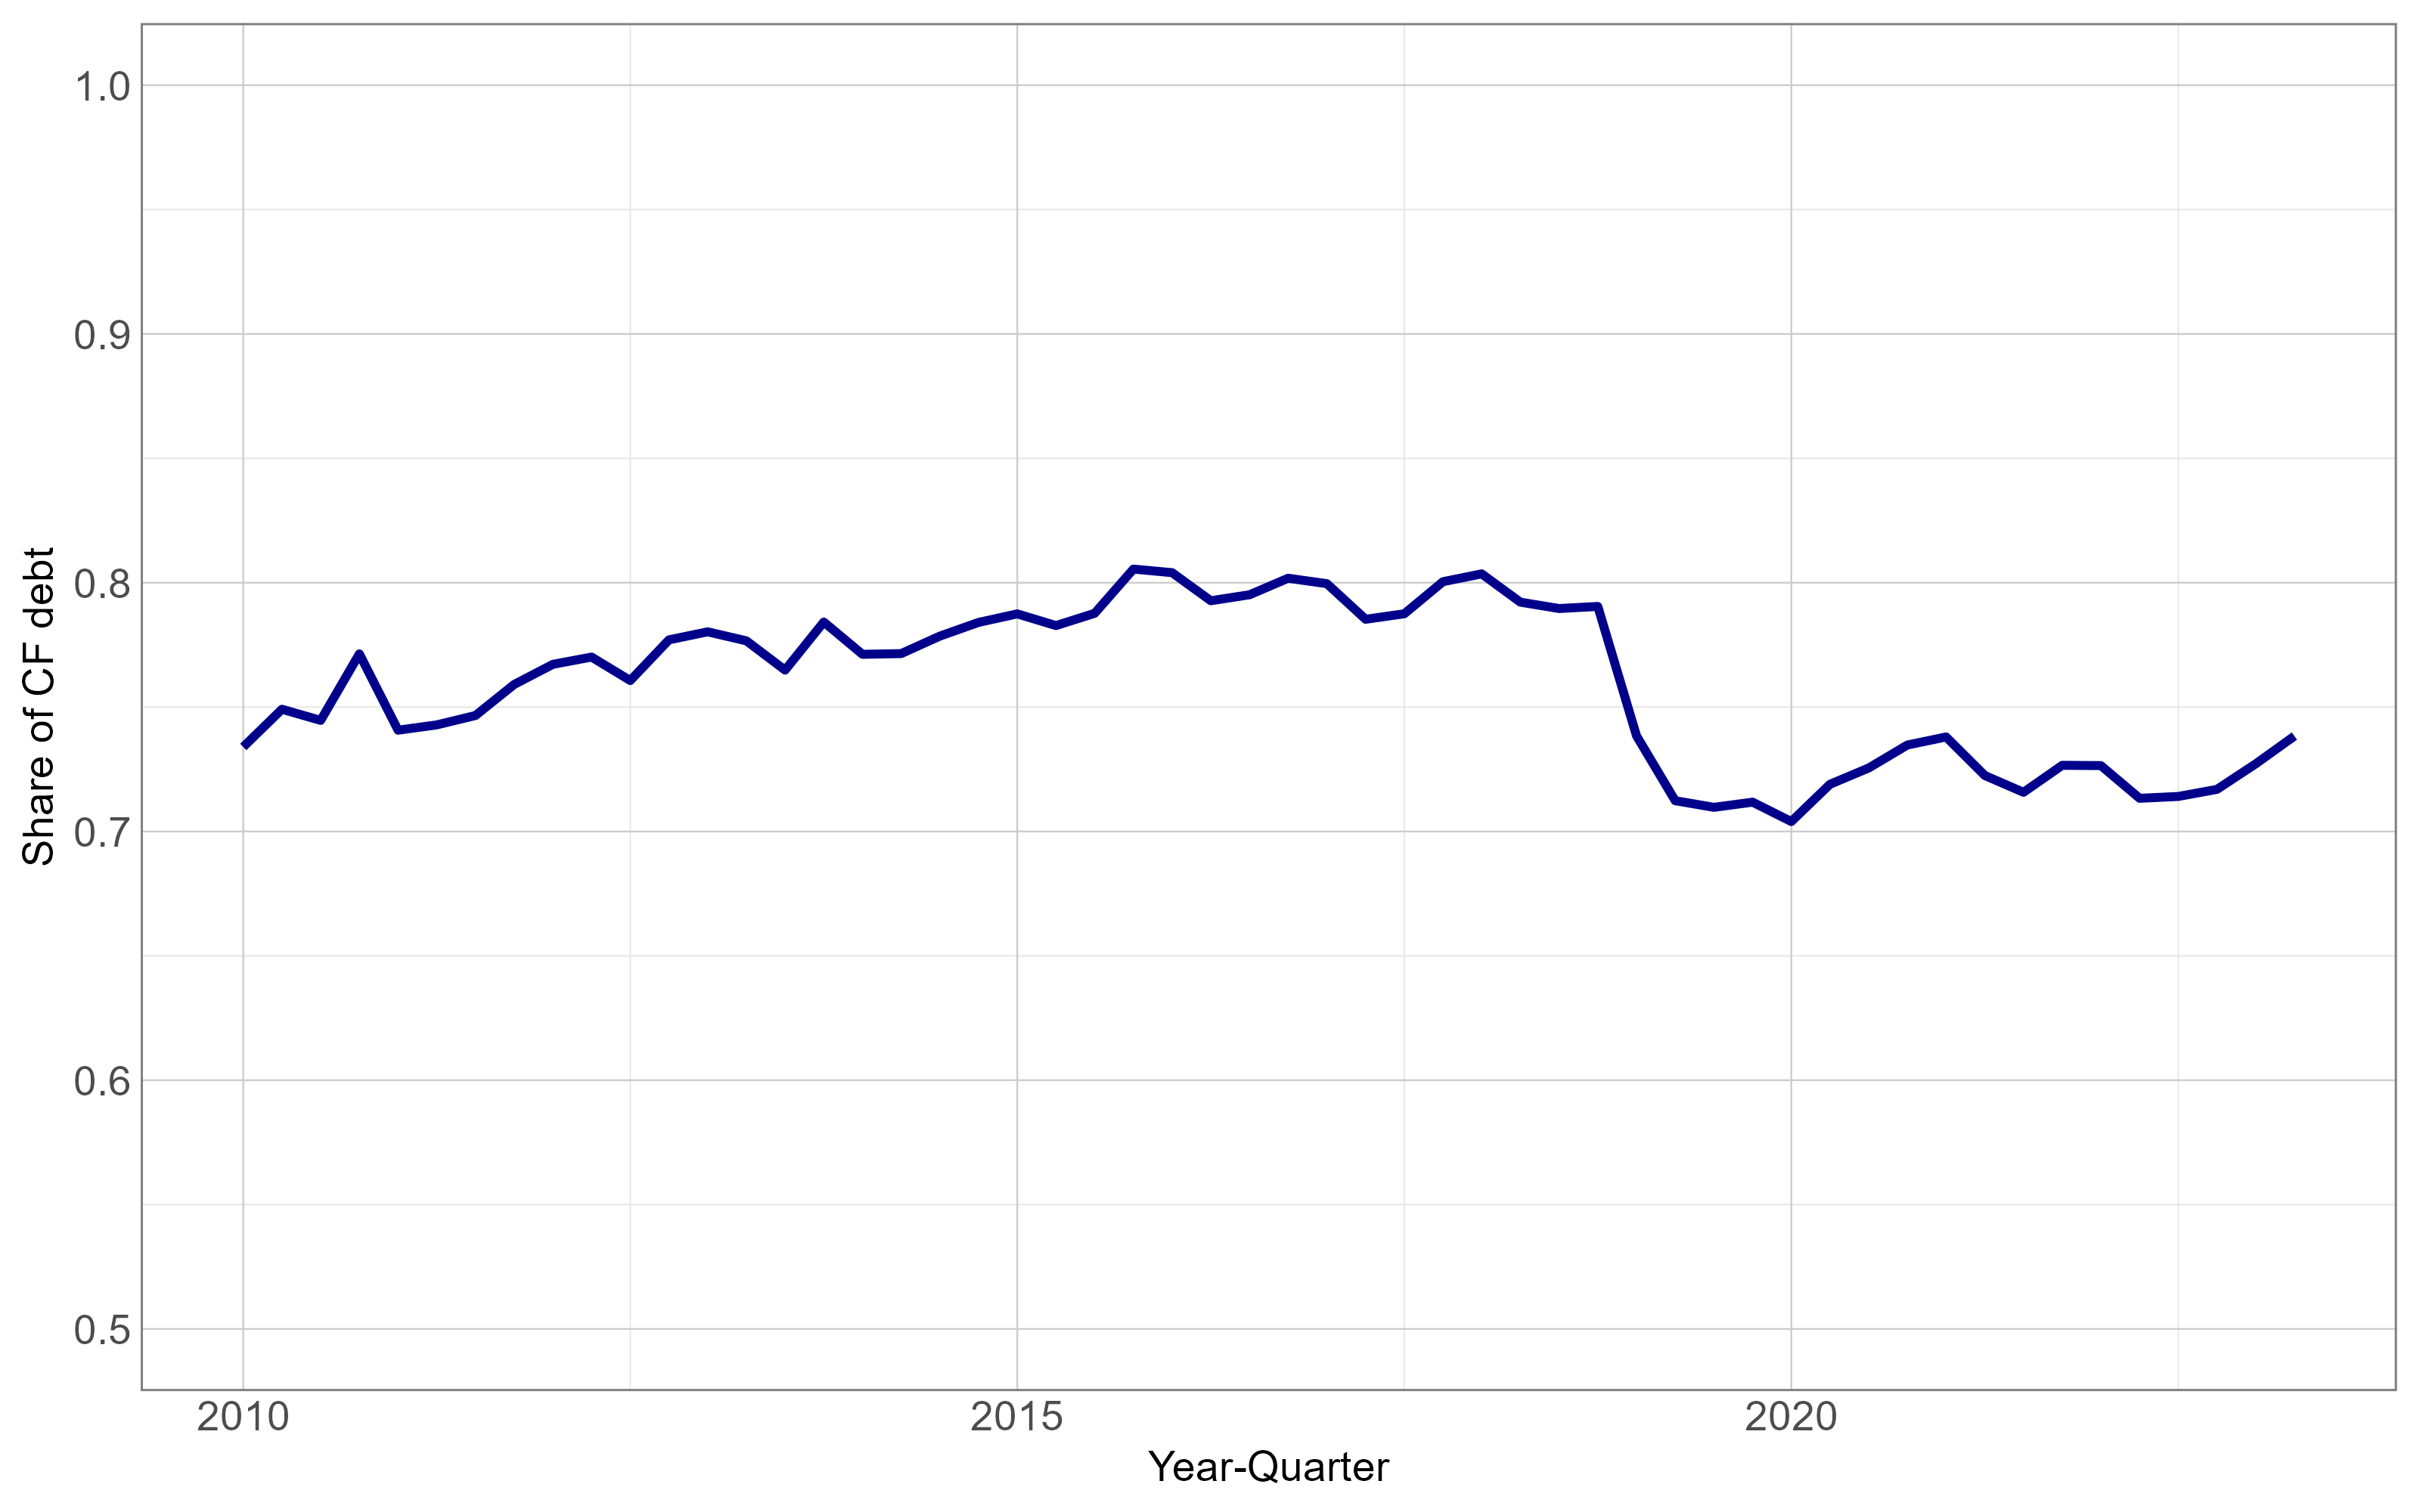
\includegraphics[width=1\textwidth]{CFshare.png}
     \small The share CFL debt to total debt, by volume between 2010Q1 and 2023Q3
\end{figure}

Figure 2. of appendix shows the share entries (red) and exits (blue) from the CFL debt market. Plotted against firm age, these show a steadily decreasing trend. Some of this might simply be down to the fact that once a firm entered the CFL market, it would have first exit to enter again. This seems relatively unlikely even though there is some churning on the extensive margin. Plotted against size, firms are most likely to enter around 1-10 million of total assets and most likely to exit at a size of 10-100 million of total assets. This is consistent with the U-shaped CFL reliance (figure 1.), which indicates that firms of this size rely on CF-based borrowing to a lesser extent. 

\begin{figure}[H]  % [h] indicates placing the image here
    \centering
    \caption{The share firms exiting and entering the CFL market}
    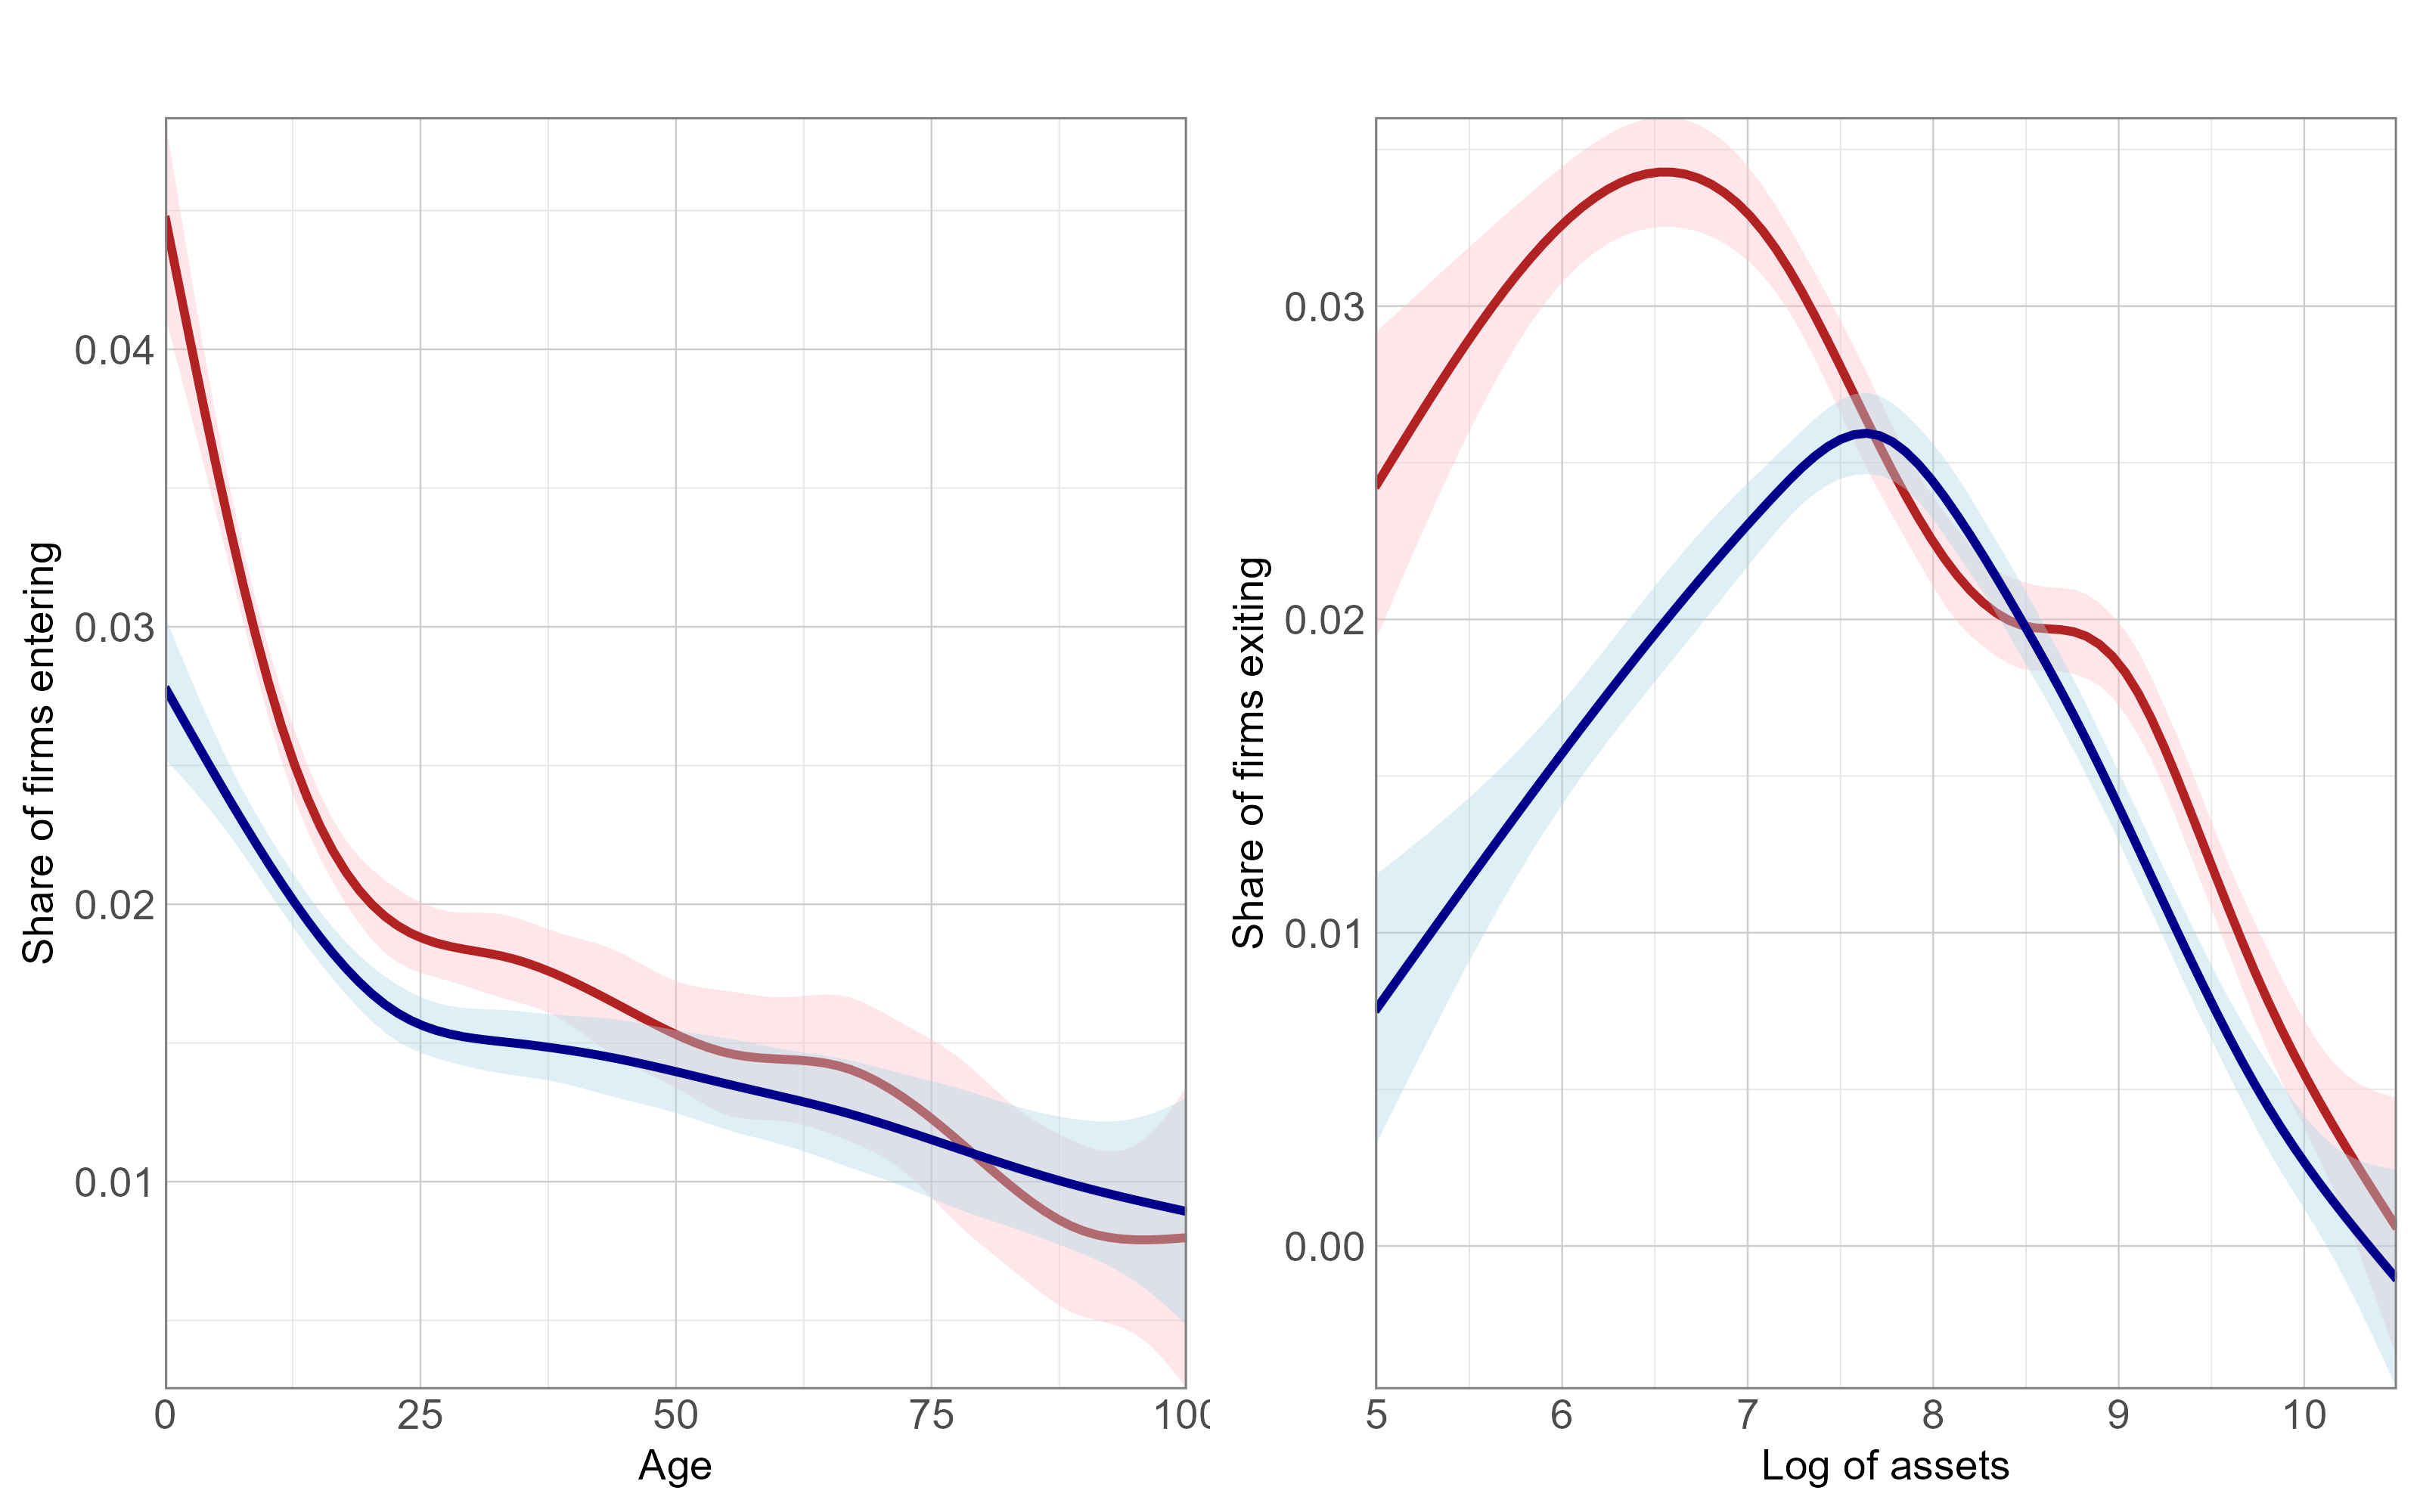
\includegraphics[width=1\textwidth]{exit_entry.png}
     \small Moving average of the probability of entering and exiting the CF-based debt market. The blue line indicates exits, whereas the red line shows entries.
\end{figure}

\newpage

\noindent Figure 3. shows a moving average of CFL reliance as a function  of different explanatory variables. Plotting this variable against revenue and the number of employees yields the same U-shape as in the case of assets. However, revenue and employees become insignificant in the multivariate analysis, once assets are taken into account. Hence, I focus on total assets in the main body of the analysis. Similarly to the multivariate analysis, leverage seems to be an important determinant of CFL reliance: the the least indebted firms, the average is close to 25\% which increases to around 75\% for the most indebted firms. Conversely, pledgeability, which is an important determinant in the multivariate analysis, does not exhibit a strong correlation with cash-flow based lending (CFL) reliance. \textbf{May worth discussing profitability too.}

\begin{figure}[H]  % [h] indicates placing the image here
    \centering
    \caption{CFL reliance in relation to the regression variables}
    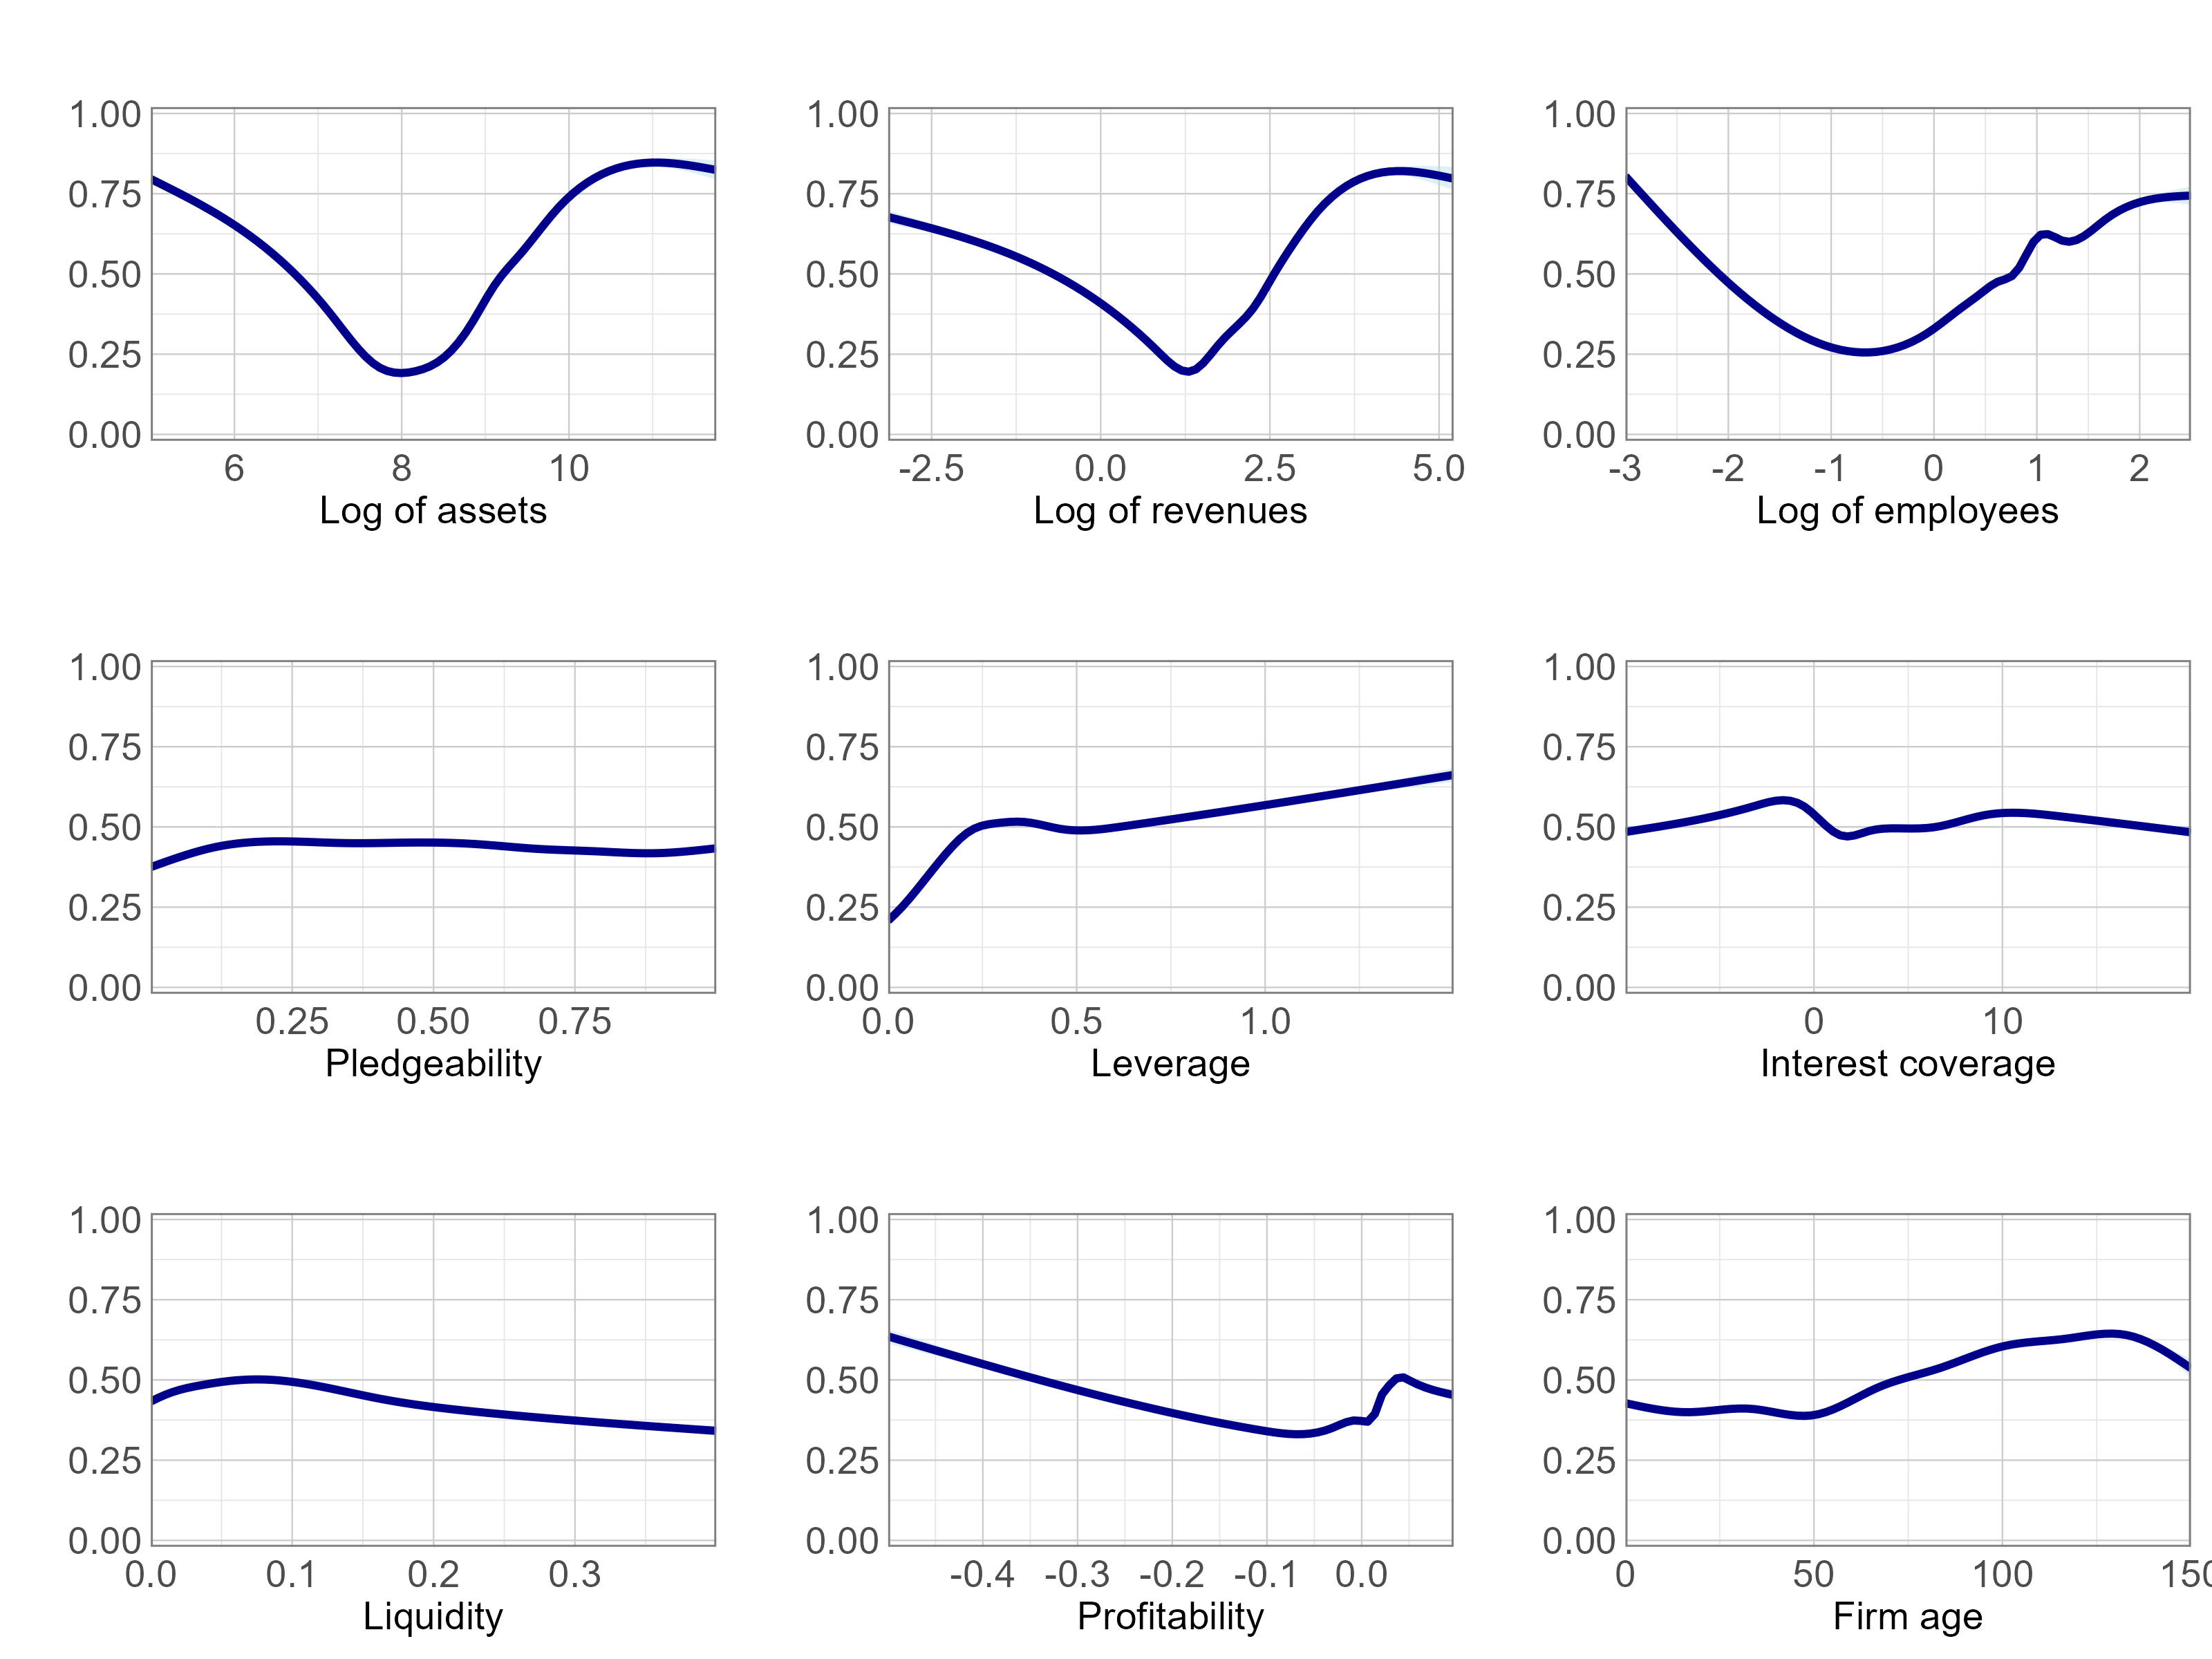
\includegraphics[width=1\textwidth]{varCFL.png}
     \small Moving average of CFL reliance in relation to other regression variables.
\end{figure}

\subsubsection*{A4.2 - Orbis and Capital IQ evidence}

In the following, I present results from the combination of Orbis and capital IQ data. I discuss the connecting these datasets in section ... . Orbis contains a wide range of traded and non-traded companies as well. However, I only have detailed debt information on firms that are included in Capital IQ, which mostly focuses on traded firms. Additionally, due to the absence of a common unique firm identifier, matching these two datasets is not perfect. Hence, this dataset is not representative of the entire population of firms in these countries. Nonetheless, it could offer valuable insights into the impacts of legal and institutional frameworks on CF-based lending, given the limited availability of cross-country evidence in existing literature. \vspace{3mm} \\
Although both CapitalIQ and Orbis contains observations from every major economies, I only discuss countries that provide a sufficient number of good quality matches. Therefore, in figure 4 and 5, I present evidence from six Asian and two North American economies only. Additionally I present `Full Sample' results, which comprise all good quality matches across the world. The first thing to discern from figure 4, is that country differences matter. In Japan, which traditionally relies on asset based debt contracts, the share of firms that only hold asset-based debt is around 70\%. On the other hand, most Taiwanese firms rely on a mix of asset-based and CF-based debt contracts, which means that only around 20\% of the holds a purely asset based debt portfolio. \textbf{Add horizontal lines for averages and discuss it.} \vspace{3mm} \\
In general, North American economies have a higher average reliance on CF based borrowing than their Asian counterparts. Lian and Ma argues that there are traditional reasons for this in Japan. For the rest of the Asian economies, lower reliance is could be down similar reasons or to differences in bankruptcy practices. In figure 5, I test the persistence of the U-shaped CFL reliance across firm sizes: it holds for the US, Canada and India as well as for the full sample. However, no discernible U-shape is observable for most Asian economies (with the exception of South Korea) where CF-based lendings is not as prevalent.

\begin{figure}[H]  % [h] indicates placing the image here
    \centering
    \caption{The cumulative distribution function of CFL reliance, across countries}
    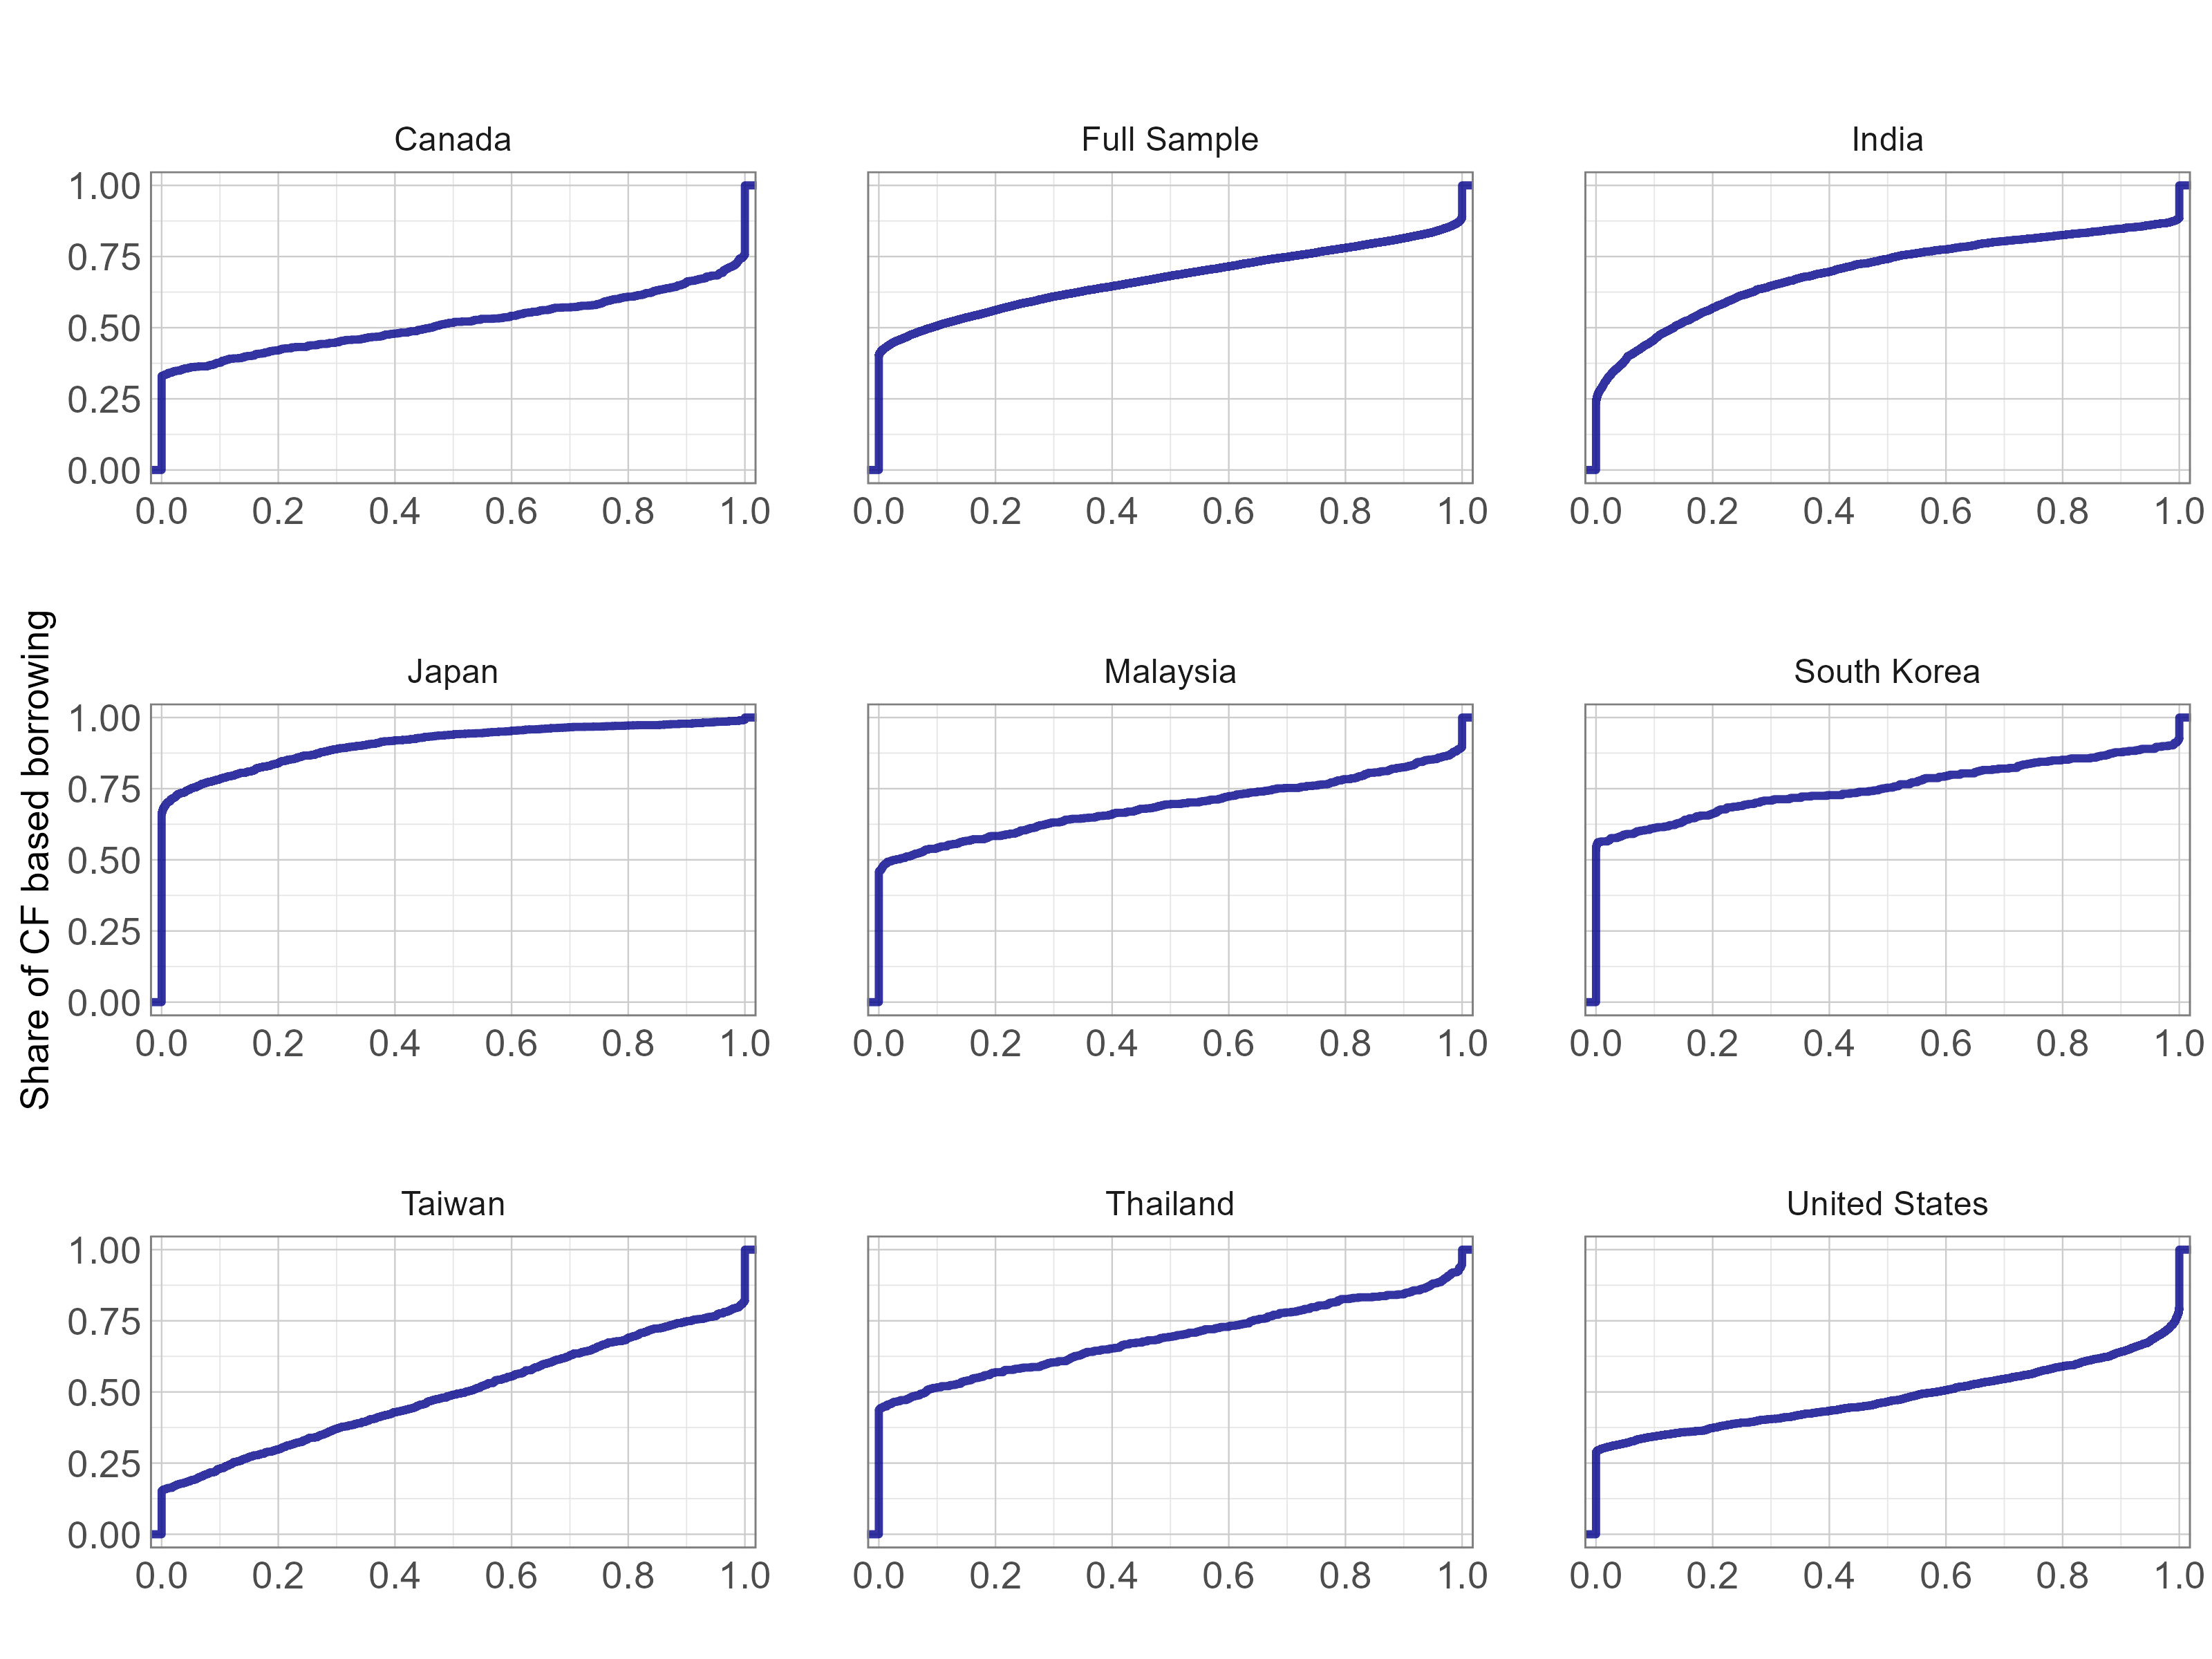
\includegraphics[width=1\textwidth]{cdf_country.png}
    \small The cumulative distribution of CFL reliance in selected economies and in the full sample
\end{figure}

\begin{figure}[H]  % [h] indicates placing the image here
    \centering
    \caption{The distribution of CFL debt over firms size, across countries}
    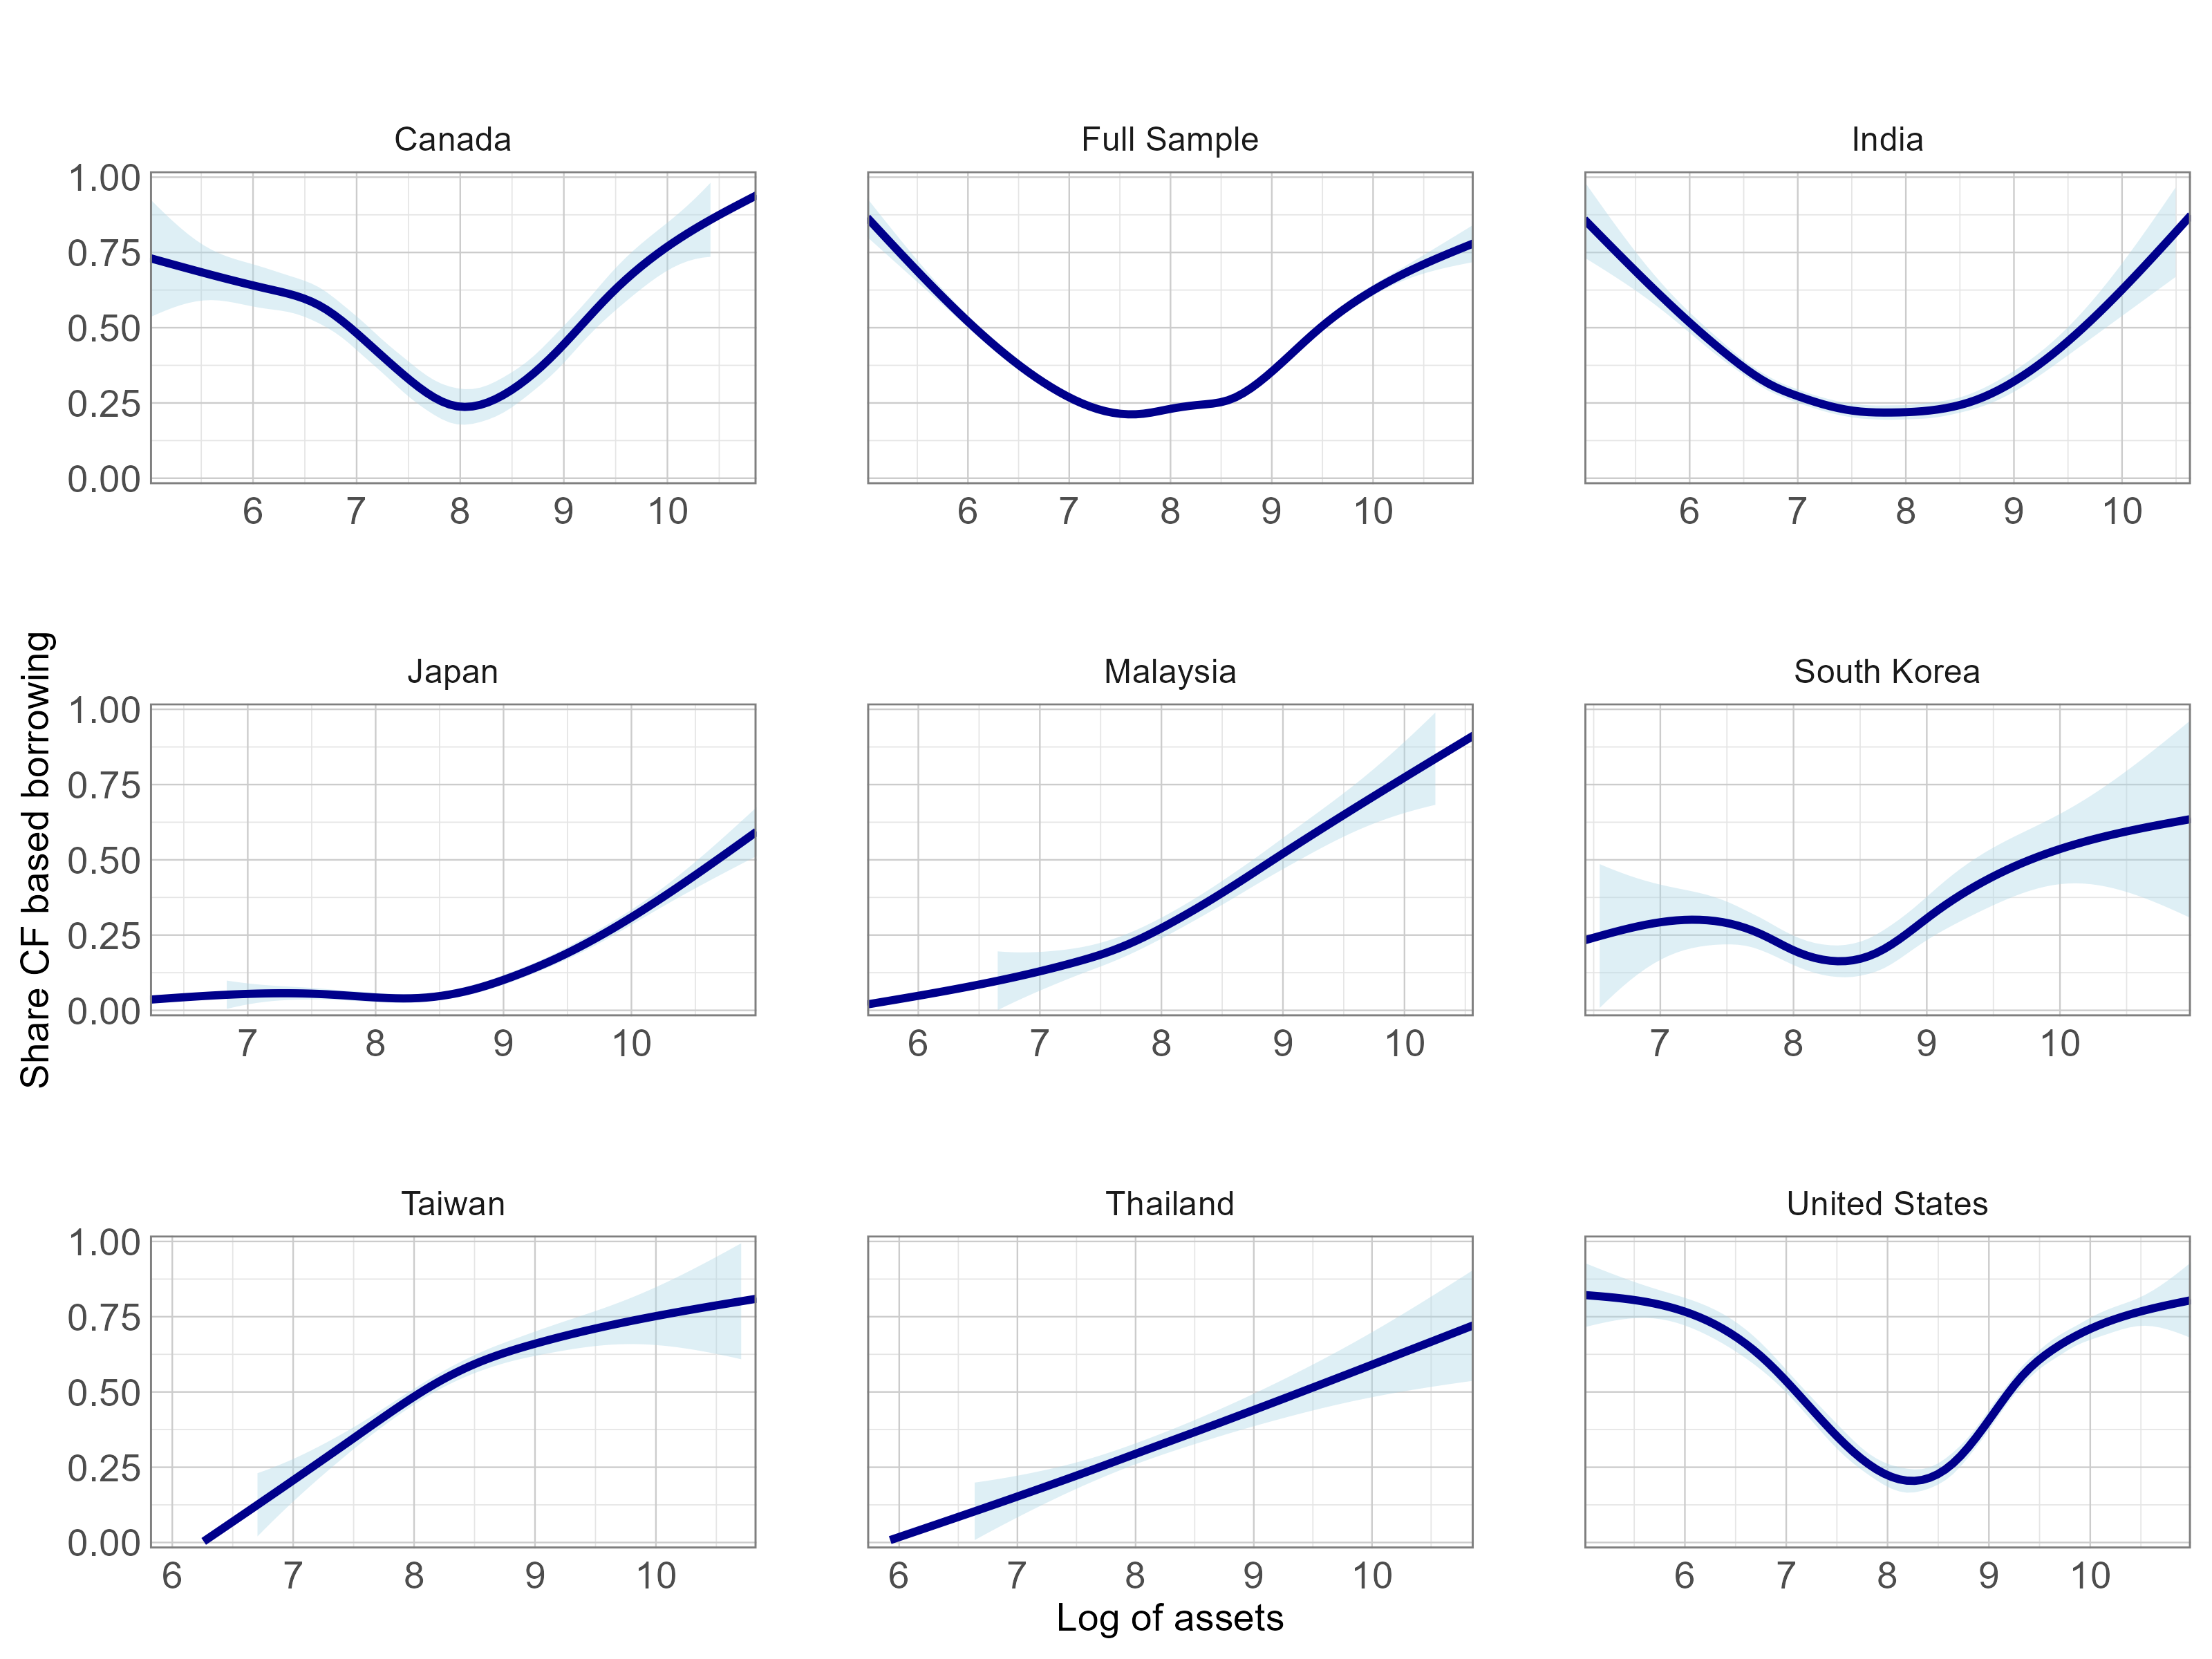
\includegraphics[width=1\textwidth]{smoothy_country.png}
    \small CFL reliance against the logarithm of assets in selected economies and in the full sample
\end{figure}


\end{document}







